% ---------- Metadata ----------
\title[Aula 8]{Aula 8 - Título da Aula}
\author[Marcato]{Professor: André L. Marcato}
\institute[UFJF]{Universidade Federal de Juiz de Fora \\ Engenharia Elétrica — Robótica e Automação Industrial}

% ---------- Title ----------
\begin{frame}
  \titlepage
\end{frame}

% ---------- Overview ----------
\begin{frame}{Roteiro}
\tableofcontents
\end{frame}

% ---------- Conteúdo ----------
% ---------- Conteúdo Aula 8 ----------
\section{Conceitos: DDS e QoS}

% --- Slide: O que é DDS? ---
\begin{frame}[fragile]{\href{https://docs.ros.org/en/humble/Concepts/About-Quality-of-Service-Settings.html}{\uline{DDS e Quality of Service (QoS)}}}
  \begin{itemize}
    \item \textbf{DDS (Data Distribution Service)}: É o \textit{middleware} padrão do ROS 2.
    \item Diferente do ROS 1 (que usava TCP/UDP fixo), o DDS permite ajuste fino da comunicação.
    \item \textbf{QoS (Quality of Service)}: Conjunto de "regras" que definem como os dados são trocados.
    \item Cenários de uso:
      \begin{itemize}
        \item Câmera de vídeo (perder frames é aceitável $\rightarrow$ \textit{Best Effort}).
        \item Comando de emergência (não pode perder $\rightarrow$ \textit{Reliable}).
        \item Mapas estáticos (quem entrar depois deve receber $\rightarrow$ \textit{Transient Local}).
      \end{itemize}
  \end{itemize}
\end{frame}

% --- Slide: Principais Políticas ---
\begin{frame}[fragile]{Principais Políticas de QoS}
  \begin{description}
    \item[History / Depth] Quantas mensagens guardar na fila?
      \begin{itemize}
        \item \textit{Keep Last (N)}: Guarda as últimas N (padrão).
        \item \textit{Keep All}: Tenta guardar tudo (cuidado com memória!).
      \end{itemize}
    
    \item[Reliability] Garantia de entrega.
      \begin{itemize}
        \item \textit{Best Effort}: "Dispara e esquece" (tipo UDP). Rápido, mas pode perder dados.
        \item \textit{Reliable}: Garante entrega (tipo TCP). Pode retransmitir se falhar.
      \end{itemize}

    \item[Durability] Persistência para "atrasados".
      \begin{itemize}
        \item \textit{Volatile}: Só recebe quem já está conectado.
        \item \textit{Transient Local}: O Publisher guarda as últimas mensagens para quem conectar depois (Late Joiner).
      \end{itemize}
  \end{description}
\end{frame}

% --- Slide: Compatibilidade (Diagrama Placeholder) ---
\begin{frame}{Compatibilidade de QoS}
  \begin{itemize}
    \item Para haver comunicação, o \textbf{Publisher} e o \textbf{Subscriber} devem ser compatíveis.
    \item Regra de Ouro: O \textit{Subscriber} não pode exigir mais "qualidade" do que o \textit{Publisher} oferece.
  \end{itemize}
  
  \centering
  % Diagrama de Compatibilidade (Prompt fornecido abaixo)
  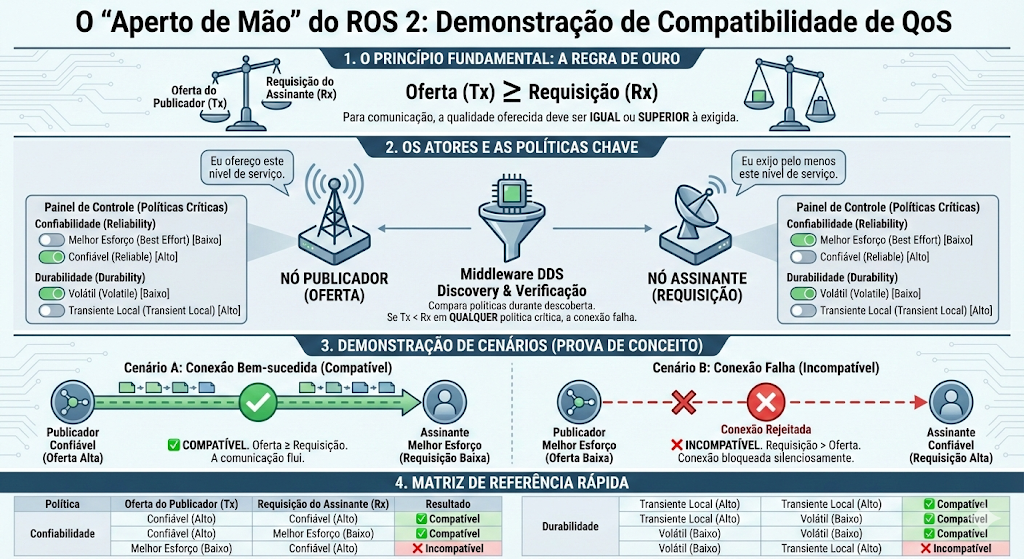
\includegraphics[width=0.8\textwidth]{aula8/images/image.png}
\end{frame}

\section{Prática: Configuração}

% --- Slide: Perfis Padrão ---
\begin{frame}[fragile]{Perfis de QoS Predefinidos}
  \begin{itemize}
    \item O ROS 2 fornece perfis comuns para facilitar.
  \end{itemize}
  
  \begin{center}
  
\includegraphics[width=0.85\textwidth]{code_qos_profiles.png}
  \end{center}
\end{frame}

% --- Slide: Exemplo Prático (Código) ---
\begin{frame}[fragile]{Aplicando QoS no Código}
  \begin{itemize}
    \item Definimos o perfil na criação do Publisher/Subscriber.
  \end{itemize}

  \begin{center}
  
\includegraphics[width=0.85\textwidth]{code_qos_apply.png}
  \end{center}
\end{frame}

% --- Slide: Inspeção CLI ---
\begin{frame}[fragile]{Inspeção via CLI}
  \begin{itemize}
    \item Problemas de comunicação? Geralmente é incompatibilidade de QoS.
    \item Use \texttt{--verbose} para ver os detalhes.
  \end{itemize}

\begin{lstlisting}[style=bashstyle]
# Ver detalhes de QoS de quem publica/escuta
$ ros2 topic info /robot_state --verbose

# Saida esperada:
# Node name: qos_demo
# QoS profile:
#   Reliability: RELIABLE
#   Durability: TRANSIENT_LOCAL
#   ...
\end{lstlisting}

  \begin{alertblock}{Atenção}
    Se Reliability do Pub for \texttt{BEST\_EFFORT} e do Sub for \texttt{RELIABLE}, eles \textbf{não} se conectam.
  \end{alertblock}
\end{frame}

% --- Slide: Exercício ---
\begin{frame}[fragile]{Exercício: O "Late Joiner"}
  \begin{enumerate}
    \item Crie um nó \textbf{Publisher} que publica uma única mensagem ("Configuração X") e depois não publica mais nada (apenas dorme).
    \item Use QoS \textbf{Transient Local}.
    \item Rode o nó.
    \item Em outro terminal (após alguns segundos), inicie um \textbf{Subscriber} (ou \texttt{ros2 topic echo}) configurado também como Transient Local.
    \item \textbf{Objetivo:} Verificar se o Subscriber recebe a mensagem antiga imediatamente ao conectar.
  \end{enumerate}
  
  \vspace{0.5em}
  \textit{Dica CLI:}
  \texttt{ros2 topic echo /topic --qos-durability transient\_local}
\end{frame}

